\chapter{Обзор предметной области}
\label{ch:chapter1}

В данной главе произведён обзор предметной области настоящего
исследования.

В разделе~\ref{sec:profiling_problem} подробно разобрана задача
профилирования пользователей, а также описана основная сложность,
возникающая при решении данной задачи.

В разделе~\ref{sec:previous_work} рассматриваются методы и
результаты, опубликованные в различных исследованиях, в рамках
которых решалась задача восстановления неизвестных характеристик
пользователей.

Наконец, в разделе~\ref{sec:problem_formulation} приведено
формальное описание задачи, решаемой в рамках настоящей
работы.

\section{Задача профилирования пользователей}
\label{sec:profiling_problem}

\textit{Задача профилирования} пользователей представляет из себя
задачу восстановления неизвестных характеристик пользователей
по известным. Часто задача профилирования решается с
использованием данных из социальных сетей, но также имеет
место возможность использовать данные из любых других
онлайн-сервисов, которые предоставляют возможности
регистрации и сохранения каких-либо данных о каждом
конкретном пользователе.

В качестве неизвестных характеристик пользователей,
которые требуется восстановить, могут выступать такие данные как пол и 
возраст (демографические характеристики)~\cite{burger2006exploration,
peersman2011predicting,turdakov2013opredelenie,schwartz2013personality,
rosenthal2011age,liu2012inferring,baluja2007boosting}. Обычно задача
определения демографических характеристик решает проблему устранения
неполноты в данных: часто многие сайты предоставляют возможность
пользователям заполнять не все поля в различных анкетах. 
Устранение неполноты в данных о демографических характеристиках
пользователей позволяет улучшить различные системы рекомендаций,
так как подобные признаки являются одними из ключевых в
рекомендательных системах~\cite{swearingen2001beyond,adomavicius2005toward}.
Задача восстановления пола и возраста пользователей, как правило,
сводится к классическим задачам машинного обучения~--- к
задаче классификации или задаче восстановления регрессионной зависимости.

Неизвестные характеристики пользователей, которые требуется
определить, также могут быть очень нетипичными. Например
авторы работы~\cite{schwartz2013personality} предлагают
подход, позволяющий выявлять психотип пользователей, основываясь
на данных из их профилей социальных сетей. Подобные исследования
востребованы в такой науке, как психология, так как метод
определения психологического портрета пользователя даёт
возможность выявлять новые закономерности и строить новые
гипотезы относительно поведения людей. Подобные задачи,
как правило, сводятся к задачам классификации, кластеризации
или регрессии.

Ещё одним распространённым типом задач профилирования является
выделение групп пользователей. В работе~\cite{barbera2015tweeting}
предлагается подход, позволяющий определять политические взгляды
пользователей, путём разбиения их на группы, что может быть
использовано в политических целях. Авторы 
работы~\cite{maia2008identifying} описывают метод, позволяющий
произвести кластеризацию пользователей, основываясь на некоторых
метриках. Кластеризация пользователей часто оказывается полезной
при реализации систем рекомендаций~\cite{sarwar2002recommender}.

В качестве информации о пользователях, на основе которой
восстанавливаются неизвестные характеристики, как правило,
может быть использована любая доступная информация. На просторах
различных социальных сетей и онлайн-сервисов доступно огромное
множество различных данных, таких как текст сообщений пользователей,
фотографии, социальные связи, активность пользователей в течение
дня, дата регистрации и многие другие.

Основная сложность, возникающая при решении конкретной задачи
профилирования, заключается в сведении задачи к задаче машинного
обучения (классификации, восстановления регрессии, кластеризации и
так далее). Требуется представить каждого пользователя в
виде вектора (на практике, как правило, численного), пригодного для
использования его алгоритмом машинного обучения, причём таким образом,
чтобы алгоритм показывал хорошие результаты. Метод построения векторной
модели, описывающей пользователей, зависит от типа данных,
которые используются. Процесс преобразования данных некоторого вида в
численные вектора иногда оказывается крайне нетривиальным шагом.

\section{Обзор существующих исследований}
\label{sec:previous_work}

Как было описано в предыдущем разделе, основной проблемой при решении
задач профилирования пользователей является построение модели
векторного пространства признакового описания пользователей.

В данном разделе будут рассмотрены известные подходы,
позволяющие преобразовать пользователей в векторы, основываясь
на персональных данных пользователей различного вида.

\subsection{Подходы, использующие информацию отличную от музыки}
\label{ssec:without_music}

Одним из наиболее часто использующихся видов данных, применяемых
для определения характеристик пользователей, является текст, который
пишут пользователи в социальных сетях. 

В работах~\cite{miller2012gender,deitrick2012gender} применяется
подход к построению векторов, описывающих пользователей, на основе подсчёта
числа буквенных \textit{N}-грамм\footnote{\textit{N}-грамма~--- 
последовательность, состоящая из \textit{N} лингвистических единиц,
идущих друг за другом подряд}, встречающихся в сообщениях. Похожий
подход использован в работе~\cite{turdakov2013opredelenie}, но
вместо буквенных \textit{N}-грамм использовались словесные. Обоснование
данного подхода зиждется на том факте, что текст имеет некоторую
семантику, которая может быть в некоторой мере описана некоторыми
частями данного текста. Часто такой подход приводит к весьма большому
числу признаков, из-за чего возникает задача выбора наиболее
информативных признаков.

В работах~\cite{rosenthal2011age,schwartz2013personality} в качестве
известных данных в задаче профилирования также
использовался текст сообщений, но признаковое описание пользователей
формировалось на основе подсчёта слов, принадлежащих некоторым
непересекающимся семантическим категориям. Основным недостатком такого подхода
является тот факт, что составление таких категорий слов, как правило,
приходится производить вручную.

В работе~\cite{sloan2013knowing} предлагается подход к определению
пола пользователей \textit{Twitter} на основе их имён (nickname).
Авторы работы используют словарь, содержащий информацию о женских и мужских
именах. Помимо очевидного недостатка, заключающегося в том, что
словарь имён требуется составлять вручную, данный подход, кроме всего,
игнорирует тот факт, что имена пользователей социальных сетей зачастую
являются псевдонимами. Кроме того, существует ряд имён универсальных
для обоих полов.

Авторы работы~\cite{farseev2015harvesting} использовали несколько
типов данных, описывающих пользователей. Текст сообщений пользователей
был преобразован в численные признаками с помощью латентного
семантического анализа (см. раздел~\ref{sec:latent_semantic_analysis}),
также признаки из текста извлекались программным средством
LIWC~\cite{pennebaker2001linguistic}. Кроме того, признаки
строились на основе геолокации пользователей и фотографий.

В исследовании~\cite{baluja2007boosting} описан способ, позволяющий
определять пол пользователей на основе их фотографий. В качестве 
численных признаков, описывающих пользователей, используются
разности значений яркости всех пар пикселей, из которых состоит
изображение пользователей (предварительно изображения сжимаются).
Данный подход имеет ряд недостатков. Во-первых, сложность
алгоритма. Во-вторых, большая размерность пространства признакового
описания. В-третьих, необходимость применения алгоритмов
распознавания лиц, точность которых ниже точности распознавания
лиц людьми.

\subsection{Подходы, использующие информацию о музыке}
\label{ssec:with_music}

Далее следует рассмотреть подходы к решению задачи профилирования
пользователей, в которых использовалась информация о музыкальных
предпочтениях, ввиду того, что разработка подхода к решению
задачи определения характеристик пользователей на основе их
музыкальных предпочтений является целью настоящего исследования.

Первой работой, которую стоит упомянуть, 
является~\cite{christenson1988genre}.
Данная работа ни коим образом не относится к анализу социальных сетей, но
в исследовании изучались музыкальные предпочтения людей в
зависимости от их гендерной принадлежности. В рамках исследования
проводился опрос среди 239 студентов. Людям предлагалось оценить каждую
музыкальную композицию из некоторого списка по пятибалльной шкале.
Было показано, что существует корреляция между предпочитаемыми
музыкальными жанрами человеком и его полом. Результат данной статьи
даёт основания полагать, что музыкальные предпочтения конкретного
человека содержат в себе некоторую <<скрытую>> информацию о нём.

В исследовании, которое описано в работе~\cite{liu2012inferring},
для определения пола и возраста пользователей использовалась информация
с сайта \textit{Last.fm}\footnote{http://www.last.fm}. Было опробовано три
способа векторного представления пользователей: на основе даты и
времени прослушивания, на основе мета-данных о музыке, на основе
анализа аудио-файлов музыкальных композиций. Первый способ
предполагает вычисление следующих признаков для каждого пользователя:
число прослушиваний в каждый из 24 часов дня, число прослушиваний
в каждый из семи дней недели, число прослушиваний в каждый из 12 месяцев
в году, доля прослушиваний в рабочее время, доля прослушиваний в июле и августе.
Способ, основанный на мета-данных о музыке, предполагает подсчёт числа
прослушиваний каждой музыкальной композиции, каждого исполнителя, а также
подсчёт числа встреч меток\footnote{Метка (tag)~--- специфичная для сайта
Last.fm информация о музыкальной композиции или исполнителе, которую
вводят сами пользователи. Метки являются короткими описаниями исполнителя 
или композиции и чаще всего характеризуют жанр или страну
исполнителей.} исполнителей и композиций. Способ, основанный на анализе
аудио-файлов музыкальных композиций, предполагает вычисление признаков
с помощью Echo Nest API~\cite{echonest} таких как темп, громкость,
<<танцевальность>> (danceability) и так далее. Было показано, что
наилучшее качество определения пола и возраста пользователей 
достигается при использовании такой мета-информации о музыке, как
название исполнителя и название композиции. Основываясь на
результатах исследования, можно сделать вывод, что названия
музыкальных композиций и исполнителей являются наиболее
информативными данными, поэтому использование этой информации
является наиболее целесообразным.

В исследовании~\cite{wu2014gender} для решения задачи определения
демографических характеристик пользователей также в качестве
источника информации использовался сайт Last.fm. Для каждого
пользователя была сохранена информация о 50 наиболее
прослушиваемых им музыкальных композициях. Основываясь 
\textit{только} на названиях исполнителей из этого списка, 
вычислялось векторное представление для каждого пользователя.
Применялось два подхода. Первый подход заключается в том, что
список исполнителей рассматривается как текстовый документ,
далее вычисляется матрица <<термин-документ>> (см.
раздел~\ref{sec:term_document_matrix}), а затем применяется
техника латентного семантического анализа для уменьшения
размерности признакового описания. Второй подход основывается
на вычислении gaussian super vector~\cite{campbell2006support}.
Авторы исследования решали задачу определения пола как задачу
бинарной классификации, а задачу определения возраста~--- как
задачу восстановления регрессии. Наилучшие результаты, которые
были достигнуты в исследовании: точность определения пола~---
78,87\%, средняя абсолютная ошибка определения возраста~--- 3,69.
Результаты данного исследования подтверждают, что в музыкальных
предпочтениях пользователей содержится <<скрытая>> информация,
описывающая пользователей.

\section{Постановка задачи настоящего исследования}
\label{sec:problem_formulation}

Задача определения характеристик пользователей в рамках настоящего
исследования будет поставлена таким же образом, как это было
сделано в исследовании~\cite{wu2014gender}.

Имеется множество пользователей. Каждый пользователь описан списком 50
(или менее, если информации недостаточно) наиболее прослушиваемых им
музыкальных композиций. Список отсортирован по убыванию числа
прослушиваний музыкальных композиций. Каждая музыкальная композиция
содержит информацию о исполнителе. При этом, предполагается, что задача
должна решаться, использую \textit{только} названия исполнителей. Для ясности
задача профилирования пользователей по их музыкальным предпочтениям
проиллюстрирована на рисунке~\ref{fig:problem_illustration}.

\begin{figure}[!h]
\caption{Задача профилирования пользователей
         по их музыкальным предпочтениям}
\label{fig:problem_illustration}
\centering
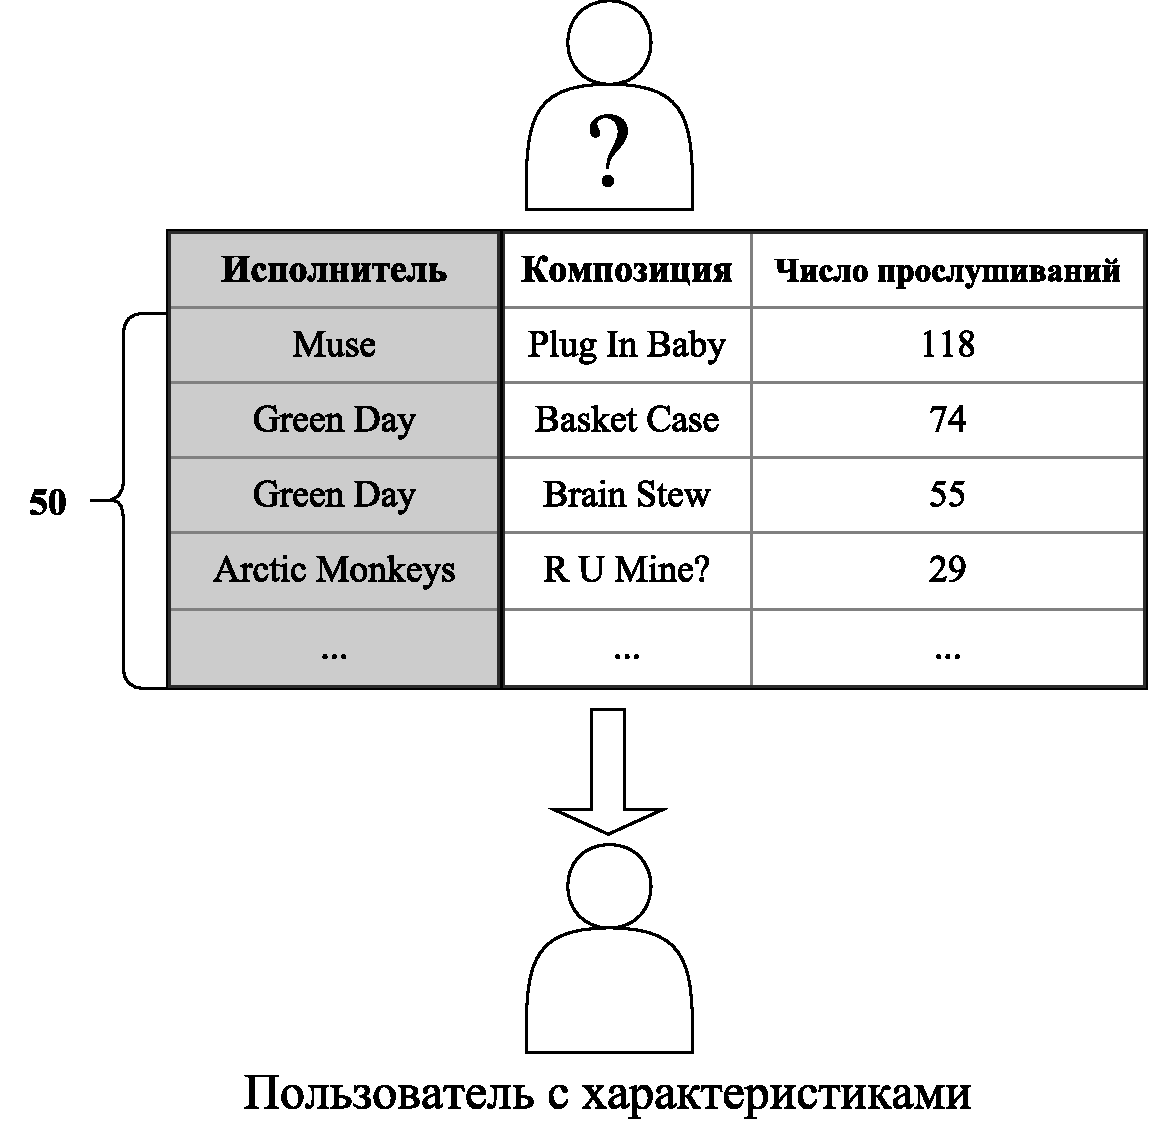
\includegraphics[scale=0.7]{figs/problem-illustration.pdf}
\end{figure}

Таким образом, каждый пользователь описан \textit{последовательностью},
каждый элемент последовательности содержит название исполнителя.
Стоит отметить, что при использовании такой информации, названия
исполнителей у одного и того же пользователя могут повторяться.

Следует указать на некоторые особенности задачи в такой постановке.
Данная задача очень похожа на задачи профилирования,
использующие текстовые данные (поэтому им был посвящён подробный обзор).
С одной стороны, список исполнителей не является полноценным текстом,
следовательно семантика, присущая текстовым сообщениям, в данной задаче
отсутствует. Поэтому подходы на основе \textit{N}-грамм или на основе
выделения частей речи в данном случае не применимы. С другой стороны,
названия исполнителей у каждого пользователя упорядочены по вполне
определённому принципу, поэтому здесь имеет место гипотеза о значимости
порядка следования исполнителей.

\chapterconclusion

В данной главе была рассмотрена задача профилирования пользователей.
Были рассмотрены исследования в рамках которых эта задача решалась.
Отдельно были рассмотрены работы, в которых восстановление
характеристик пользователей производилось на основе их музыкальных
интересов. Наконец, была описана задача, решаемая в
рамках настоящего исследования.
